People use a number of nonverbal cues to shape the footing of conversational participants. Two important ones are body orientation and eye gaze. People orient their bodies toward core participants (speakers and addressees), such that they maintain a conversational formation with them. They also distribute their gaze among them, gazing mostly toward the core participants and only infrequently toward bystanders.
In this section, I introduce computational models for synthesis of these behaviors on virtual agents.
The body reorientation model performs shifts of the agent's body orientation toward new addressees joining the interaction in order to reconfigure the conversational formation.
The gaze model performs shifts of the agent's eye gaze among the core participants and bystanders according to probability distributions derived from previous work~\citep{mutlu2012conversational}.
The movements that comprise these behaviors---body orientation shifts and eye gaze shifts---are kinematically similar, as they both involve coordinated reorienting of the eyes, head, and (in some cases) body toward targets in the environment. We synthesize both types of movements using the gaze shift model from Chapter~\ref{cha:GazeShiftModel}. This section concludes with an overview of the models' prototype implementation in an embodied, multiparty dialog system.

\subsection{Body-Reorientation Model}

When two people interact, they typically face each other directly, creating a so-called vis-a-vis arrangement, though they may also stand at a 90$^\circ$ angle, in an L-shape formation~\citep{kendon1990conducting}. When there are more than two participants in a conversation, they generally stand in a circular formation. \citet{kendon1990conducting} has coined the term ``F-formation'' to refer to these spatial arrangements of interacting participants. The F-formation serves as a footing cue---speakers and addressees are a part of it, while bystanders are not.

In order to correctly establish conversational footing, a virtual agent must be able to maintain an F-formation with other participants. When a new addressee approaches the agent, the latter must turn toward the newcomer to reconfigure the F-formation. Likewise, when a current participant leaves, the agent may need to reorient itself toward the remaining participants. Here, we describe a model for synthesis of body orientation shifts that achieve correct F-formation reconfiguration.

\begin{figure}
\centering
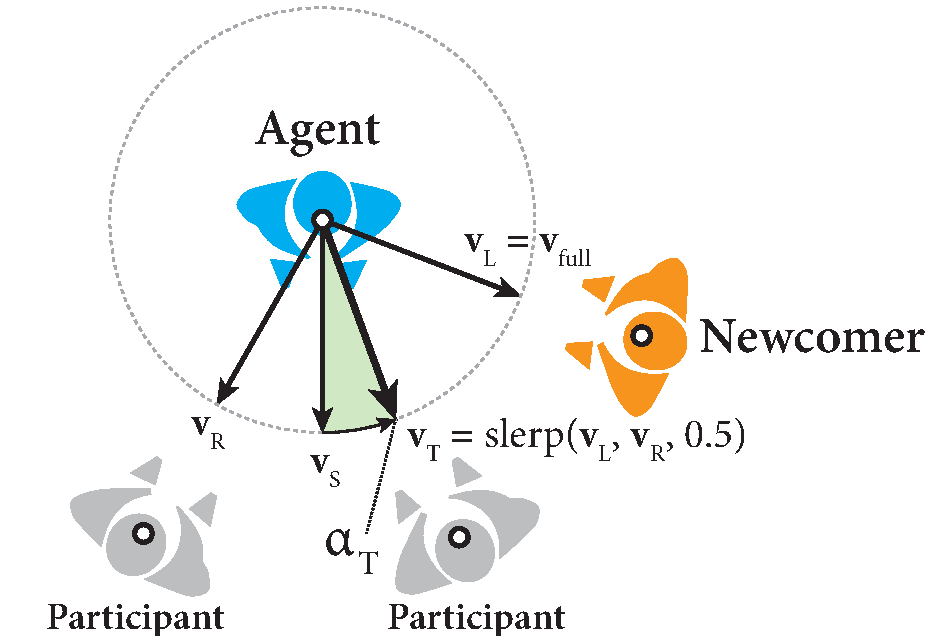
\includegraphics[width=0.75\textwidth]{conversationalrolegaze/Figures/FTorsoAlign.pdf}
\caption{Computing the torso alignment parameter $\alpha_T$ needed for the agent to reconfigure the F-formation when a new user has joined the interaction.}
\label{fig:FTorsoAlign}
\end{figure}

We use our gaze shift model (Chapter~\ref{cha:GazeShiftModel}) to synthesize the agent's body orientation shifts. When the first participant approaches the agent, the agent performs a gaze shift toward the participant with the head, torso, and whole-body alignment parameters all set to 1 ($\alpha_H = \alpha_T = \alpha_B = 1$). This results in the agent facing the participant head-on. If participants are already present in the interaction, the agent must perform a gaze shift toward the new participant that evenly distributes its body orientation among all the participants. We set $\alpha_H = 1$ and $\alpha_B = 1$ as before, whereas $\alpha_T$ must be set such that the agent ends up oriented toward the midpoint between the leftmost and rightmost participant. The procedure for computing $\alpha_T$ is as follows (Figure~\ref{fig:FTorsoAlign}). Let us define the following direction vectors:

\begin{itemize}
\item $\mathbf{v}_S$ -- Current torso facing direction of the agent.
\item $\mathbf{v}_T$ -- Target torso facing direction of the agent.
\item $\mathbf{v}_\mathrm{full}$ -- Torso facing direction which would fully align the agent with the new user.
\item $\mathbf{v}_L$ -- Direction vector from the agent to the leftmost user.
\item $\mathbf{v}_R$ -- Direction vector from the agent to the rightmost user.
\end{itemize}

All direction vectors are projected onto the horizontal plane. The agent must realign its body such that its torso facing direction ends up the following: $\mathbf{v}_T = \mathop{slerp}(\mathbf{v}_L, \mathbf{v}_R, 0.5)$. The function $\mathop{slerp}$ denotes interpolation between two direction vectors. It can be computed by rotating $\mathbf{v}_L$ toward $\mathbf{v}_R$ by $0.5 \phi_{LR}$, where $\phi_{LR}$ is the angle between the direction vectors. The torso alignment $\alpha_T$ needed to achieve the facing direction $\mathbf{v}_T$ is:
%
\begin{align} \label{eq:FTorsoAlign}
\alpha_T = \frac{\angle(\mathbf{v}_S, \mathbf{v}_T)}{\angle(\mathbf{v}_S, \mathbf{v}_\mathrm{full})}
\end{align}
%
An analogous mechanism can be used to reestablish the F-formation when a participant departs or moves. This is only required when either the leftmost or the rightmost participant has departed. If that should happen, the agent performs a body orientation shift toward the participant on the opposite end of the formation, with $\alpha_T$ computed as described above.

\subsection{Eye Gaze Model}

Participants' footing is also reflected in their gaze behavior. The current speaker uses gaze to indicate the addressees of the utterance or to release the floor to them, while the addressees gaze toward the speaker to display attentiveness. As a result, speakers and addressees gaze toward each other most of the time, while bystanders receive little gaze by comparison. \citet{mutlu2012conversational} report the gaze distributions of human speakers engaging in three types of interactions: with one addressee, two addressees, and one addressee with one bystander. According to their data, when there is a single addressee, the participants spend only 26\% of the time looking at the addressee's face (making eye contact), while the rest of the time they avert their gaze toward the addressee's torso and the environment. The gaze aversions serve the purpose of intimacy regulation---eye contact is an arousal stimulus and staring into another person's eyes for long periods of time is known to cause discomfort~\citep{argyle1976gaze}. When a second addressee is present, the amount of gaze toward each addressee's face remains in the neighborhood of 26\%, but there is much less torso-directed gaze. This is likely because switching gaze among the addressees now also achieves the purpose of intimacy regulation. Finally, if a bystander is present, participants only gaze at them 5\% of the time, or one fifth of the addressee gaze amount.

We build our footing gaze model based on the distributions reported by~\citet{mutlu2012conversational}, with the difference that our model is designed to generalize to interactions with larger groups of addressees and bystanders. Our model defines a discrete probability distribution over the set of gaze targets, which includes the faces and torsos of all the addressees and bystanders, as well as the environment. The distribution is characterized by a probability mass function $p_T = p(T, N_A, N_B)$ (Table~\ref{tab:GazeFootingSpatial}). The function $p_T$ specifies the probability of looking at the candidate target $T$ (addressee face or torso, bystander face or torso, or the environment) given the current configuration of participant footing. The footing configuration is specified by the number of addressees, $N_A$, and the number of bystanders, $N_B$. As the agent speaks or waits for a participant to take the floor, it continually shifts its gaze between targets, which are chosen by drawing from $p_T$ (Table~\ref{tab:GazeFootingSpatial}). The temporal duration of each gaze fixation is then determined by drawing from a set of gamma distributions given in Table~\ref{tab:GazeFootingFixationLengths}, also derived from previous work~\citep{mutlu2012conversational}. While the exponential distribution is more commonly used to model events that occur at a constant average rate---such as gaze shifts---we find that the gamma distribution better describes human gaze. Unlike the exponential distribution, the gamma distribution assigns a low probability to very short fixations, which are unlikely due to human motor limitations.

\begin{table}[t]
\small
\centering
\def\arraystretch{1.5}
\begin{tabular}{lrr}
\hline
\textbf{Gaze Target} & \textbf{Footing Configuration} & \textbf{Gaze Probability} \\
\hline
\multirow{2}{*}{Addressee \emph{face}} & $N_A = 1$ & 26\% \\
& $N_A \geq 2$ & $54\%/N_A$ \\
\hdashline
\multirow{2}{*}{Addressee \emph{torso}} & $N_A = 1$ & 48\% \\
& $N_A \geq 2$ & $16\%/N_A$ \\
\hdashline
\multirow{2}{*}{Bystander \emph{face}} & $N_B = 1$ & 5\% \\
& $N_B \geq 2$ & $8\%/N_B$ \\
\hdashline
\multirow{2}{*}{Bystander \emph{torso}} & $N_B = 1$ & 3\% \\
& $N_B \geq 2$ & $5\%/N_B$ \\
\hdashline
\multirow{6}{*}{Environment} & $N_A = 1$, $N_B = 0$ & 26\% \\
& $N_A = 1$, $N_B = 1$ & 18\% \\
& $N_A = 1$, $N_B \geq 2$ & 13\% \\
& $N_A \geq 2$, $N_B = 0$ & 30\% \\
& $N_A \geq 2$, $N_B = 1$ & 24\% \\
& $N_A \geq 2$, $N_B \geq 2$ & 17\% \\
\hline
\end{tabular}
\caption{Spatial probability distribution of the speaker's gaze, given as the probability of looking toward a target in the given configuration of conversational roles. $N_A$ is the number of addressees, while $N_B$ is the number of bystanders.}
\label{tab:GazeFootingSpatial}
\end{table}

\begin{table}[t]
\small
\centering
\def\arraystretch{1.5}
\begin{tabular}{llr}
\hline
\textbf{Gaze Target} & \textbf{Footing Configuration} & \textbf{Fixation Length} \\
\hline
\multirow{3}{*}{Addressee \emph{face}} & $N_A = 1$, $N_B = 0$ & $\mathop{Gamma}(1.65, 0.56)$ \\
& $N_A = 1$, $N_B = 1$ & $\mathop{Gamma}(0.74, 1.55)$ \\
& $N_A \geq 2$ & $\mathop{Gamma}(1.48, 1.10)$ \\
\hdashline
\multirow{3}{*}{Addressee \emph{torso}} & $N_A = 1$, $N_B = 0$ & $\mathop{Gamma}(1.92, 0.84)$ \\
& $N_A = 1$, $N_B = 1$ & $\mathop{Gamma}(1.72, 1.20)$ \\
& $N_A \geq 2$ & $\mathop{Gamma}(1.92, 0.52)$ \\
\hdashline
Bystander \emph{face} & $N_B \geq 1$ & $\mathop{Gamma}(2.19, 0.44)$ \\
\hdashline
Bystander \emph{torso} & $N_B \geq 1$ & $\mathop{Gamma}(1.76, 0.57)$ \\
\hdashline
\multirow{3}{*}{Environment} & $N_A = 1$, $N_B = 0$ & $\mathop{Gamma}(0.90, 1.14)$ \\
& $N_A = 1$, $N_B = 1$ & $\mathop{Gamma}(1.84, 0.59)$ \\
& $N_A \geq 2$ & $\mathop{Gamma}(2.23, 0.41)$ \\
\hline
\end{tabular}
\caption{Agent's gaze fixation lengths (in seconds), expressed as gamma distributions specifying the length of fixation of a target in the given configuration of conversational roles.}
\label{tab:GazeFootingFixationLengths}
\end{table}

Consider the following example: the agent is speaking with two addressees ($N_A = 2$) named Alice and Bob, with two bystanders present ($N_B = 2$). When the time comes to shift the agent's gaze, we draw from the spatial probability distribution to determine the target of the gaze shift. According to Table~\ref{tab:GazeFootingSpatial}, the probability of looking at Alice's face is $54\% / 2 = 27\%$ (second row); let us assume this is the target we have chosen by drawing from the distribution. We supply the chosen target to the gaze shift model, which performs a gaze shift toward Alice's face. We hold the agent' gaze there for a duration determined by drawing from the distribution $\mathop{Gamma}(k = 1.48, \Phi = 1.10)$ (Table~\ref{tab:GazeFootingFixationLengths}, third row).

\subsubsection{Environment-Directed Gaze}

It is also possible that by drawing from the distribution we determine that the next target should be in the environment. However, Table~\ref{tab:GazeFootingSpatial} does not tell us \emph{where} in the environment that target is located---it only tells us the probability of looking \emph{anywhere} within the environment. How do we determine the exact target of an environment-directed gaze aversion? Such gaze aversions are meant to be brief glances away from the current addressee, rather than large gaze shifts toward a new attentional focus. For this reason, the gaze aversion target is chosen such that it lies in the proximity of the current addressee. More formally, we predefine a set of $n$ target locations around each participant, located to their left, right, and front (at their feet). We label these locations $\mathbf{p}_{E,i}$, where $i = [1..n]$. If by drawing from the spatial probability distribution we have determined that the agent's next gaze shift is an environment-directed aversion, we choose with uniform probability among the $n$ candidate locations around the \emph{currently gazed-at addressee}. Let us assume we have chosen the $k$-th location. We determine the exact 3D position of the target, $\mathbf{p}_E$, by drawing from a clipped, spherical normal distribution centered on $\mathbf{p}_{E,k}$: $\mathbf{p}_E = \mathbf{p}_{E,k} + N(0, \sigma = R/2)$. $R$ is the radius of the sphere around $\mathbf{p}_{E,i}$ to which the normal distribution is clipped---we set $R$ to 37 cm in our model.

\subsubsection{Supporting Additional Participants}

\citet{mutlu2012conversational} only provide data for interactions with two addressees or one addressee and one bystander. However, we want to design a more robust gaze model that supports interactions with larger groups of participants. We extrapolate the original distributions~\citep{mutlu2012conversational} to configurations with 3+ addressees and 2+ bystanders. Our extrapolated distribution is based on the idea that the total probability of the agent looking at addressees is a constant 70\%. This probability is then equally divided among individual addressees, so if $N_A = 3$, the probability of looking at any one addressee is 23\%. The latter probability is the sum of probabilities of looking at the addressee's face (18\%) versus their torso (5\%). It implicitly follows from Table~\ref{tab:GazeFootingSpatial} that the ratio of face and torso probabilities is also constant. By the same token, we extrapolate the probabilities of looking at bystanders. If we have 2+ bystanders, the total probability of looking at them is a constant 13\%, which gets equally divided among them.

We believe that our gaze model generalizes well to small groups of participants with arbitrary footing configurations. In larger groups, it is likely that the total proportion of gaze toward addressees increases, while gaze toward the environment and bystanders may decay toward zero. Additional data collection is required to build a model for large-scale multiparty interactions.

\subsection{System Design and Implementation}

We implemented the footing behavior models within a prototype system for embodied, multiparty dialog. Here, we give an overview of the system in order to illustrate how our models might be utilized in practice.

The gaze and body-orientation models are implemented within a \emph{behavior controller} used in conjunction with a high-level dialog management module. The dialog manager performs the tasks needed to conduct multiparty dialog: it keeps track of participants joining and leaving, as well as their conversational roles; it receives and interprets the participants' utterances from the speech recognizer; and it plans the agent's dialog acts. We use five types of dialog acts: \emph{ParticipantJoin}, \emph{ParticipantLeave}, \emph{Speak}, \emph{WaitForSpeech}, and \emph{Listen}. Each dialog act is associated with nonverbal behaviors and speech utterances, which are produced by the behavior controller and rendered on the virtual embodiment.

\emph{ParticipantJoin} and \emph{ParticipantLeave} acts are generated when a participant joins or leaves the interaction. If the participant is an addressee rather than a bystander, the behavior controller triggers a body orientation shift to reconfigure the conversational formation using the mechanism described earlier in the section. When a \emph{Speak} act occurs, the behavior controller renders a speech utterance addressed at one or more participants. Once the agent has completed its utterance, a \emph{WaitForSpeech} act is generated, during which the agent is releasing the floor to one or more participants. During the production of \emph{Speak} and \emph{WaitForSpeech} acts, the behavior controller generates the agent's gaze behavior according to our footing gaze model; it directs the agent's gaze toward the current addressees, with occasional glances toward bystanders and the environment. When one of the participants begins the speak, a \emph{Listen} act is generated, during which the agent's gaze fixates upon the speaker, with frequent gaze aversions generated by an implementation of the model by~\citet{lee2002eyes}

Our system is implemented in Unity game engine. System components such as the behavior controller, gaze shift model, and dialog manager are all implemented as Unity C\# scripts. The system uses Microsoft Speech SDK to detect and recognize users' speech utterances, and to synthesize the agent's speech. The visemes generated by the Speech SDK are used to animate the agent's lip movements. 